%!TEX root = <../index.tex>

\section{Experimental Results and Discussion}
\label{sec:5}

The experimental results are described, analyzed and concluded in this section. In section \ref{sec:5.1} the statistics of the corpus after preprocessing is showed briefly. Section \ref{sec:5.2} focuses on the effectiveness of the different STS models, i.e. how precisely the STS models judge an articles as related for a given target article. Furthermore, the operational performance of the STS models is reported in section \ref{sec:5.3}. The above three parts concentrate on the results of the first experiment, which is mentioned in section \ref{sec:4.4}. On the next step, the results of the second experiment are reported in section \ref{sec:5.4}. After reporting the results of the both experiments, we discuss the most severe types of errors that an articles which is virtually unrelated is judged as related for a target article or a cluster of articles which are properly related are never or rarely judged as related. In conclusion, we summarize the consequence of selection of the STS models and the challenge of the current work. 

\bigbreak

\subsection{Analysis of Preprocessing}
\label{sec:5.1}

Each article contains three semantic components, so-called text sources, including \icontent{}, \ititle{}, \isummary{} which are as input data of the framework. After preprocessing the text sources in raw string format is converted to a sequence of words which consist of $n$ tokens. 

\begin{figure}[!htb]
    \centering
    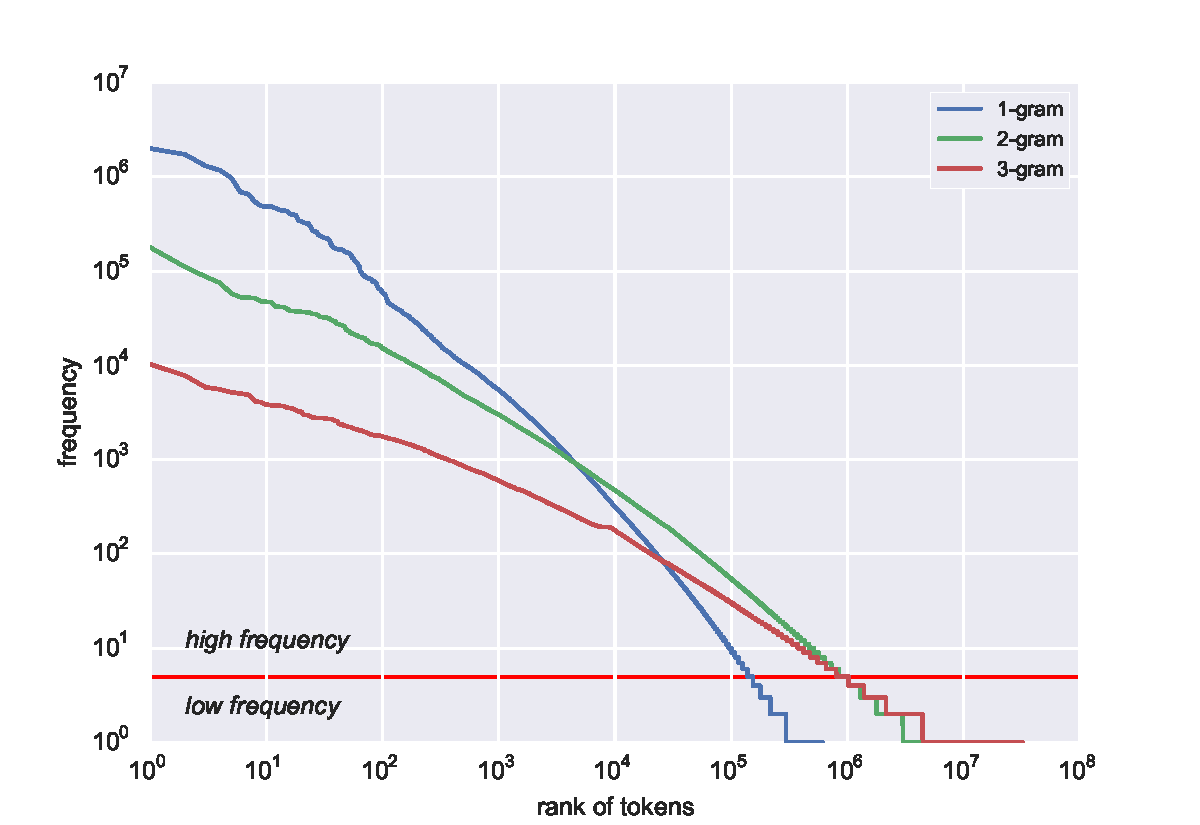
\includegraphics[width=0.8\textwidth]{fig/freqdist}
    \caption{Occurrence Frequencies of terms in the corpus for uni-, bi- and trigram in descending ranking. The applied preprocessing method is \iSE{} and the text source is \icontent{}.}
    \label{fig:freqdist}
\end{figure}

\begin{figure}[!htb]
    \centering
    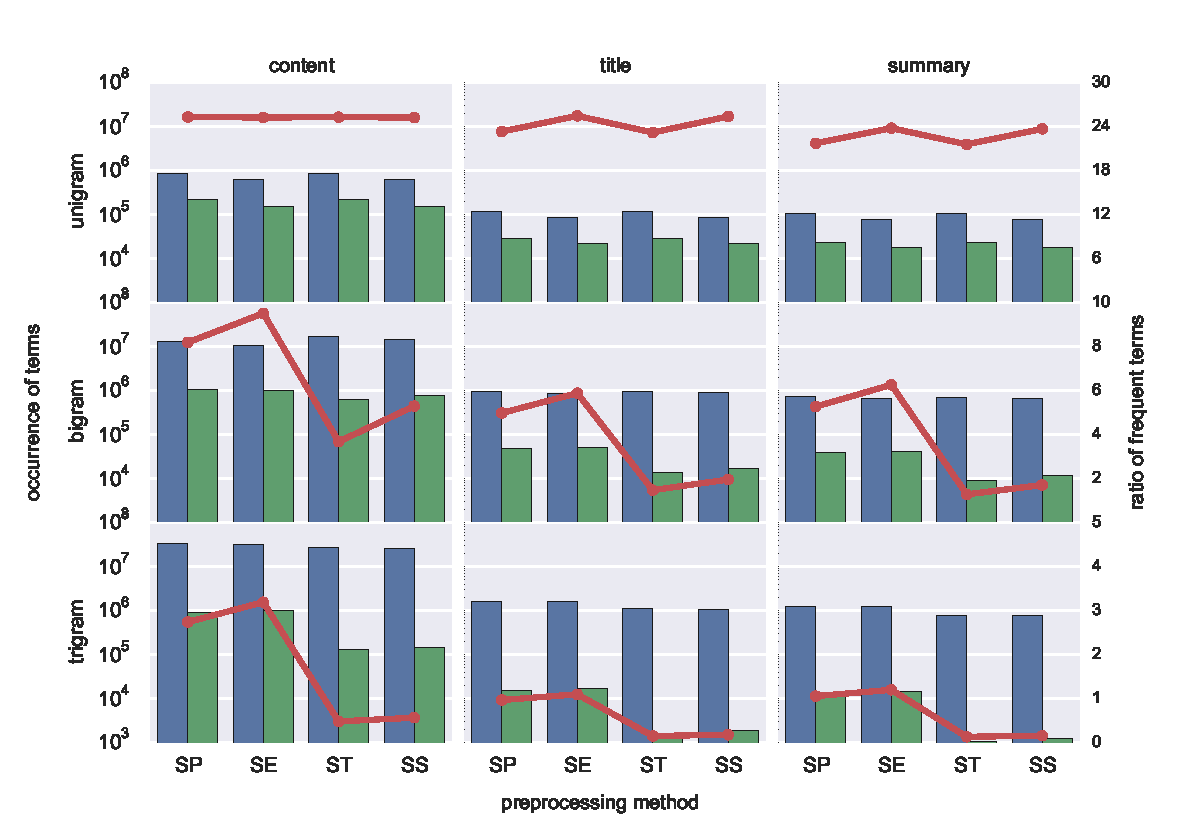
\includegraphics[width=\textwidth]{fig/vocab_size}
    \caption{Compare the vocabulary size of all text fields over n-gram models.}
    \begin{tabular}{|ll|} \hline \textbf{Legend} & \\ Column & types of text fields; \icontent{}, \ititle{} and \isummary{}, respectively \\ Row & corresponding n-gram models; uni-, bi-, trigram, respectively \\ Blue bars & \ifull{} vocabularies containing all terms \\ Green bars & \icommon{} vocabularies retaining frequently used terms \\ Red lines & the ratio of the size of \icommon{} vocabularies to the size of corresponding \\ & \ifull{} vocabularies. \\ \hline \end{tabular}
    \label{fig:vocab_size}
\end{figure}


There are two attributes to portray a vocabulary. The first attribute is the size, which decides the computation complexity, such as the dimension of vector space. The second one is the scale of ``long tail'' of the vocabulary. The ``long tail'' is the part of the distribution which contains a large number of elements with low occurrence frequency. In our case, the threshold of ``long tail'' is $5$, in other words, the terms occurring less than $5$ times belong to the ``long tail'' of the vocabulary. According to the Zipf's law, the occurrence frequency is distributed extremely unevenly or that is to say that the most terms are rarely in use and hence it is almost incapable of determining the semantic relevance of these terms by statistical methods. In ideal case, a vocabulary with smaller size and fewer low-frequency terms has the better quality of operational complexity and semantic completeness. Figure \ref{fig:freqdist}, which depicts the representative distribution of the occurrence frequency of terms, indicates that only a small quantity of tokens occur repetitively in the corpus (25\% for unigram, 10\% for bigram and 3\% for trigram). In respect of efficiency, the tokens which appear less than $5$ times can be removed from the vocabulary. We denote the original vocabularies as \ifull{} vocabularies and the reduced vocabularies as \icommon{} vocabularies. 



We consider the size of \ifull{} vocabularies and the proportion of frequent tokens as the metrics to evaluate the vocabulary quality. Figure \ref{fig:vocab_size} shows the comparison between the size of \ifull{} and \icommon{} vocabularies which are generated by the preprocessing methods including \iSP{}, \iSE{}, \iST{} and \iSS{} in the different n-gram models ($n=1, 2, 3$) of the three types of text source containing \icontent{}, \ititle{} and \isummary{}. In the unigram model, \iSS{} always generates the vocabularies with the smallest size and the largest proportion of frequent terms. In bi- and trigram, the vocabularies generated by \iSE{} have the largest proportion of frequent terms and the size is slightly different with the vocabularies generated by other methods. In conclusion, the preprocessing method \iSS{} is applied for preprocessing using the unigram model and \iSE{} is applied for preprocessing using the bigram and trigram models in the application. 


\subsection{Effectiveness of STS Models}
\label{sec:5.2}


As described in section \ref{sec:3.3}, the indicators of effectiveness are \textit{precision@k@h} to evaluate the relatedness of the articles in the top positions and \textit{nDCG} to evaluate the overall results. First, the results for each PF are given and the best STS methods are selected. We give in advance the reasonable assumption that an article is definitively (or ``true'') related to the articles which are not further than $3$ hops in the related-graph. Later in this part, the divergence between different categories is discussed and for which categories the framework is more suitable are concluded.  


\subsubsection{Parameter Selection for Topic Models}

Topic models, such as LSI and LDA, represent documents as vectors in the topic space. The dimension of the topic space, as well as the number of topics is pre-defined. Hence, it is necessary to determine the optimal number of topics before building and evaluating models. Figure \ref{fig:precision_topics} shows the plot of precision and operational time of LSI along with increasing the number of topics in the range of $50 \sim 1000$. The systems are generated with $73908$ training data and then discover related articles for $2000$ randomly selected articles. In the left subfigure, the dash lines indicate the building time and the solid lines indicate the sum of building time and total predicting time. On one side, the precision keeps monotone increasing  but the growth rate decreases, as the number of topics becomes larger. On the other side, the time cost of building and predicting increases with a relative stable growth rate. Taking the reasonable limitation of time in the experiments into account, we select $500$ as the value of this hyperparameter. The reason is the growth rate of precision is lower than $0.4\%$ per $100$ topics, if the number of topics is more than $500$, and we expect that the building time is limited to one hour and the predicting time is up to less than one second. 

\clearpage

\begin{figure}[!htb]
    \centering
    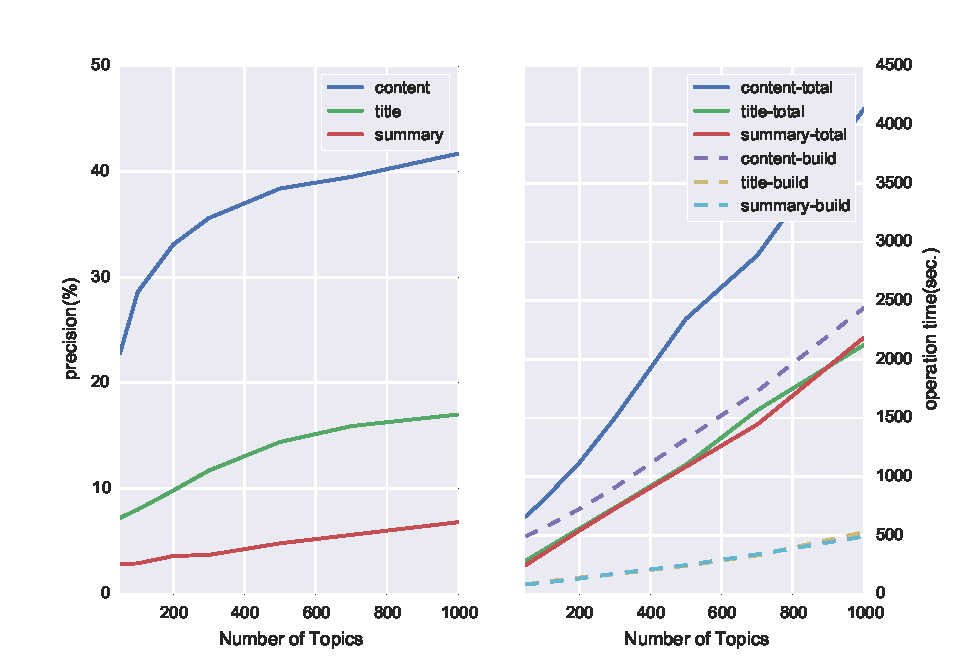
\includegraphics[width=\textwidth]{fig/precision_topics}
    \caption[Compare the effectiveness and efficiency of the system using LSI with different topic numbers from $50$ to $1000$.]{Compare the effectiveness and efficiency of the system using LSI with different topic numbers from $50$ to $1000$. The left sub-figure illustrates  \textit{precision@2@3} for all text fields over unigram and the right sub-figure the time cost in model building and in the entire process. }
    \label{fig:precision_topics}
\end{figure}

\subsubsection{Overall Analysis of Effectiveness}

\begin{figure}[!htb]
    \centering
    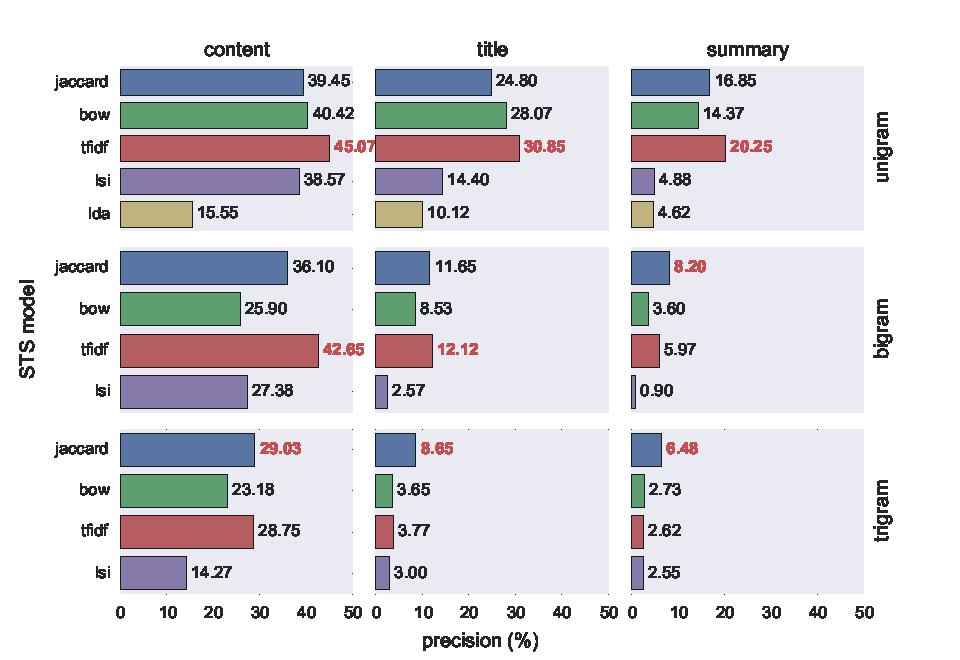
\includegraphics[width=\textwidth]{fig/precision_2_3}
    \caption[Compare \textit{precision@2@3} (\%) of Jaccard, BoW, \textit{tfidf}, LSI and LDA for all text fields over n-gram models.]{Compare \textit{precision@2@3} (\%) of Jaccard, BoW, \textit{tfidf}, LSI and LDA for all text fields over n-gram models. The value with red color refers to the precision of the best STS methods for the preprocessed text field. }
    \label{fig:precision_2_3}
\end{figure}

Figure \ref{fig:precision_2_3} compares the precision of the STS models in the different PFs. In general, all methods perform in \icontent{} better than in \ititle{} and the methods perform in \ititle{} perform better than in \isummary{}. Besides, the precision of the system using unigram model is better than using bigram model and the precision of the system using trigram is the worst. In more detail, \textit{tfidf} provides the highest precision for all text fields in unigram and for \icontent{} and \ititle{} in bigram. In the meanwhile, \textit{Jaccard} is stronger than the other STS methods for \isummary{} in bigram and all text fields in trigram. \textit{LDA} is unexpectedly the weakest method all the time in the experiment and it is discarded for evaluation in bigram and trigram. Comparing the different n-gram models for the particular text field, we find that the precision of \textit{Jaccard} fluctuates most slightly and the precision of LSI decreases with the greatest rate, in contrast. 


Figure \ref{fig:ndcg} illustrates the comparison of \textit{nDCG}, which is applied as the supplementary evaluation method. The \textit{nDCG} performance of STS methods is similar to the results of \textit{precision} in general. All STS methods are capable of effective sorting articles according to the relatedness degree, since the measure \textit{nDCG} of every method is better than the baseline. The baseline \textit{nDCG} is computed from the random order of all candidates. In more detail, LSI performs better in metric \textit{nDCG} than in metric \textit{precision} for the data source \icontent{}. To be specific, LSI is almost always in the second position after tfidf in \textit{nDCG}, while LSI is in the third or the last position in \textit{precision}. LSI computes the more precise relatedness of the overall corpus than \textit{Jaccard} and BoW, but LSI is not able to determine precisely which articles have the highest relatedness. 


Combining the results of two evaluation methods, we conclude as follows.

\begin{itemize}
\item[1] The methods using short documents, such as \ititle{} are worse than the methods using long documents like \icontent{}. 

\item[2] \textit{Title} is better than \isummary{}.

\item[3] In n-gram, the vocabulary becomes larger and the relevance between phrases become weaker along with a greater $n$. On the other hand, a higher $n$ leads to the larger loss of semantic information with removing the low-frequency terms from the vocabulary. A typical example is that $77\%$ information/phrases are lost through reducing vocabulary for \icontent{} in trigram. 

\item[4] \tfidf{} is in the dominant position for uni-/bigram and long documents, and jaccard is more suitable in trigram and short documents. LDA has the unexpected unsatisfied performance. The research of LDA is in the future work.
\end{itemize}
 

\begin{figure}[!htb]
    \centering
    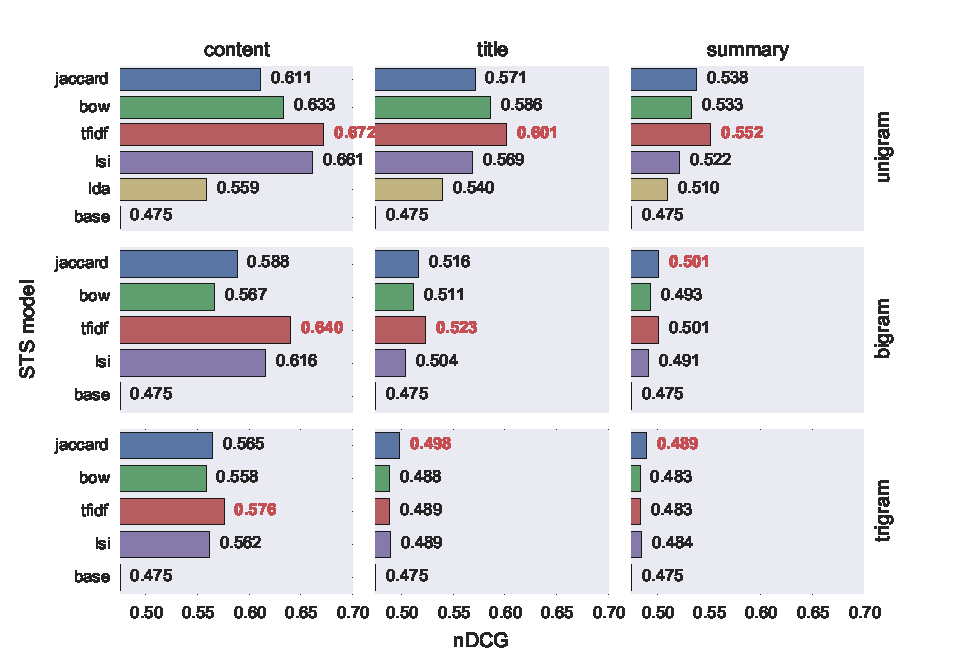
\includegraphics[width=\textwidth]{fig/ndcg}
    \caption[Compare \textit{nDCG} of Jaccard, BoW, \textit{tfidf}, LSI and LDA for all text fields over n-gram models]{Compare \textit{nDCG} of Jaccard, BoW, \textit{tfidf}, LSI and LDA for all text fields over n-gram models. The legend is the same to figure \ref{fig:precision_2_3}}
    \label{fig:ndcg}
\end{figure}

\subsubsection{Coverage of Predictions in Related-Graph}

In this part, we pay attention how the selections of related articles by the different STS methods are distributed over the related graph. We analyze the performance of the methods through comparing for each single method \textit{precision@2@h}, where $h$ can be $1$, $2$, $3$, $5$, $8$ and $10$. Here we only discuss the performance over \icontent{}, because the methods over other text fields cannot be applied alone in the system due to the low precision. 

Table \ref{tab:hops} reports \textit{precision@2@h} of the STS methods for \icontent{} over n-gram models. The random baseline is the precision of random selections. Meanwhile, the baseline means the average proportion of the number of $h$-hop neighbors for each target article to the size of candidate corpus. For example, $21.64\%$ articles in the candidate corpus are related in $10$-hops to a target article in average. For unigram, the best method for $10$-hop is LSI, of which precision is about 4 times as much as the baseline. In addition, the ranking of LSI increases along with increasing $h$. More detailed, LSI takes the fourth place of all methods for $1$-hop in all n-gram models, and it wins the first, second and third place for $10$-hop in uni-, bi- and trigram, respectively. Combining this regularity with the analysis of nDCG, we consider that LSI is good at distinguishing related articles from unrelated articles but not so good at differentiating the relatedness degree of the related articles. 

\begin{table}[!htb]
\centering
\small
\begin{tabularx}{\textwidth}{XX|XXXXXX}
\textbf{n-gram} & \textbf{STS} & \textbf{1-hop} & \textbf{2-hop} & \textbf{3-hop} & \textbf{5-hop} & \textbf{8-hop} & \textbf{10-hop} \\ \hline

\multicolumn{2}{c|}{\textbf{Random Baseline}} & 6.0E-5& 2.2E-4 & 6.8E-4 & ~~0.47 & ~~5.65 & 21.64 \\ \hline

\multirow{5}{*}{\textbf{unigram}} & Jaccard & 19.68 & 31.90 & 39.45 & 51.63 & 69.28 & 80.15 \\
 & BoW & 19.80 & 32.55 & 40.43 & 53.33 & 71.00 & 81.28 \\
 & tf-idf & \textbf{22.55} & \textbf{37.25} & \textbf{45.08} & \textbf{57.90} & 73.45 & 82.33 \\
 & LSI & 17.33 & 29.83 & 38.58 & 53.35 & \textbf{73.93} & \textbf{84.40} \\
 & LDA & ~~5.80 & 11.08 & 15.55 & 26.08 & 45.50 & 62.48 \\ \hline
\multirow{4}{*}{\textbf{bigram}} & Jaccard & 17.53 & 29.43 & 36.10 & 47.28 & 63.23 & 74.50 \\
 & BoW & 12.13 & 20.75 & 25.90 & 35.68 & 50.90 & 64.58 \\
 & tf-idf & 21.50 & 35.00 & 42.65 & 56.20 & 71.93 & 81.70 \\
 & LSI & 11.53 & 20.65 & 27.38 & 42.28 & 64.40 & 77.63 \\ \hline
\multirow{4}{*}{\textbf{trigram}} & Jaccard & 14.25 & 23.83 & 29.03 & 38.33 & 52.80 & 64.48 \\
 & BoW & 10.95 & 18.48 & 23.18 & 31.83 & 46.85 & 60.15 \\
 & tf-idf & 13.48 & 22.93 & 28.75 & 39.60 & 56.00 & 68.30 \\
 & LSI & ~~4.63 & ~~9.78 & 14.28 & 24.25 & 43.60 & 60.88 \\ \hline
\end{tabularx}
\caption[\textit{Precision@2@h} (\%) of STS methods for \icontent{} over n-gram models, where $1, 2, 3, 5, 8 \text{and} 10$ can be assigned to $h$]{\textit{Precision@2@h} (\%) of STS methods for \icontent{} over n-gram models, where $1, 2, 3, 5, 8 \text{and} 10$ can be assigned to $h$. The random baseline is computed with random selection of the candidate corpus. Two candidates for each target are selected randomly and \textit{precision@2@h} is computed as the normal way. }
\label{tab:hops}
\end{table}

\subsubsection{Divergence between Categories}

\begin{table}[!htb]
\centering
\resizebox{\textwidth}{!}{%
\begin{tabular}{lrr|rr|rr|rr|rr|rr|rr|rr|rr}
 & \multicolumn{6}{c|}{\textbf{Content}} & \multicolumn{6}{c|}{\textbf{Title}} & \multicolumn{6}{c}{\textbf{Summary}} \\
 & \multicolumn{2}{c|}{\textbf{1-tfidf}} & \multicolumn{2}{c|}{\textbf{2-tfidf}} & \multicolumn{2}{c|}{\textbf{3-jaccard}} & \multicolumn{2}{c|}{\textbf{1-tfidf}} & \multicolumn{2}{c|}{\textbf{2-tfidf}} & \multicolumn{2}{c|}{\textbf{3-jaccard}} & \multicolumn{2}{c|}{\textbf{1-tfidf}} & \multicolumn{2}{c|}{\textbf{2-jaccard}} & \multicolumn{2}{c}{\textbf{3-jaccard}} \\
 & \multicolumn{1}{c}{\textbf{r}} & \multicolumn{1}{c|}{\textbf{prec}} & \multicolumn{1}{c}{\textbf{r}} & \multicolumn{1}{c|}{\textbf{prec}} & \multicolumn{1}{c}{\textbf{r}} & \multicolumn{1}{c|}{\textbf{prec}} & \multicolumn{1}{c}{\textbf{r}} & \multicolumn{1}{c|}{\textbf{prec}} & \multicolumn{1}{c}{\textbf{r}} & \multicolumn{1}{c|}{\textbf{prec}} & \multicolumn{1}{c}{\textbf{r}} & \multicolumn{1}{c|}{\textbf{prec}} & \multicolumn{1}{c}{\textbf{r}} & \multicolumn{1}{c|}{\textbf{prec}} & \multicolumn{1}{c}{\textbf{r}} & \multicolumn{1}{c|}{\textbf{prec}} & \multicolumn{1}{c}{\textbf{r}} & \multicolumn{1}{c}{\textbf{prec}} \\ \hline
\textbf{Mean} & & 45.07 & & 42.65 & & 29.03 & & 30.85 & & 12.12 & & 8.65 & & 20.25 & & 8.20 & & 6.48 \\ \hline

\textbf{\textcolor{blue}{Digital}} & 1 & 52.21 & 2  & 46.90 & 7  & 19.03 & 1  & 38.50 & 5  & 13.72 & 7  & 6.64 & 3  & 22.12 & 6  & 6.64 & 8  & 4.42 \\
\textbf{\textcolor{blue}{Wissen}} & 2 & 50.98 & 3  & 46.08 & 4  & 23.86 & 2  & 35.62 & 9  & 7.52 & 9  & 6.54 & 7  & 17.32 & 9  & 5.56 & 10  & 3.59 \\
\textbf{\textcolor{blue}{Gesellschaft}} & 3  & 49.02 & 4  & 45.59 & 2  & 34.07 & 3  & 35.54 & 4  & 13.73 & 2  & 13.24 & 2  & 23.28 & 2  & 10.54 & 2  & 9.31 \\
\textbf{\textcolor{blue}{Politik}} & 4  & 48.79 & 1  & 48.86 & 1  & 41.18 & 4  & 33.00  & 6  & 12.73 & 5  & 9.25 & 1  & 23.54 & 3  & 9.53 & 3  & 7.18 \\
\textbf{Karriere} & 5  & 48.04 & 7  & 37.25 & 8  & 16.67 & 5  & 30.39 & 10  & 6.86 & 6  & 6.86 & 6  & 17.65 & 8  & 5.88 & 4  & 6.86 \\
\textbf{Kultur} & 6  & 42.69 & 6  & 38.58 & 9  & 13.93 & 6  & 29.91 & 1  & 17.58 & 4  & 9.36 & 4  & 21  & 4  & 9.36 & 5  & 6.85 \\
\textbf{Sport} & 7  & 41.80 & 5  & 38.93 & 5  & 23.77 & 7  & 25.82 & 3  & 16.39 & 8  & 6.56 & 5  & 18.44 & 5  & 7.79 & 6  & 6.15 \\
\textbf{Wirtschaft} & 8  & 38.44 & 8  & 35.18 & 3  & 25.24 & 8  & 24.92 & 8  & 7.65 & 10  & 6.35 & 8  & 17.10 & 7  & 6.51 & 7  & 5.70 \\
\textbf{\textcolor{red}{Reisen}} & 9  & 31.45 & 9  & 29.03 & 10  & 13.71 & 10  & 20.16 & 7  & 9.68 & 3  & 9.68 & 10  & 7.26 & 10  & 4.03 & 9  & 4.03 \\
\textbf{\textcolor{red}{Lebensart}} & 10  & 29.31 & 10  & 27.59 & 6  & 20.69 & 9  & 22.41 & 2  & 17.24 & 1  & 13.79 & 9  & 13.79 & 1  & 12.07 & 1  & 10.34 \\
\textbf{\textcolor{red}{Studium}} & 11  & 17.57 & 11  & 21.62 & 11  & 9.46 & 11  & 17.57 & 11  & 4.05 & 11  & 5.41 & 11  & 5.41 & 11  & 1.35 & 11  & 1.35 \\ \hline

\end{tabular}%
}
\caption[Comparison between \textit{precision@2@3} (\%) of different categories and the mean precision of the entire corpus]{Comparison between \textit{precision@2@3} (\%) of different categories and the mean precision of the entire corpus. \textbf{r} refers to the ranking of precision in all categories and \textbf{prec} indicates the precision for the specific category}
\label{tab:cate_precision}
\end{table}


The effectiveness is reported and analyzed above in general. Now we are also interested, how the methods, which are selected as the best for each preprocessed text field (PF) respectively, work for specific categories. The results are drawn in table \ref{tab:cate_precision}, where the precision ranking of each category and the difference ratio to the mean precision of the entire corpus are revealed. \textit{Gesellschaft} (\textit{society}) and \textit{Politik} (\textit{politics}) surpass the mean precision in all PFs. On the contrary, \textit{Wirtschaft} (\textit{economics}), \textit{Reisen} (\textit{traval}) and \textit{Studium} (\textit{study}) are the worst performed categories. The precision of these three categories is much lower than the mean level. For example, the precision of the best category (\textit{Digital}) in \icontent{}-unigram is about three times greater than the precision of the weakest category (\textit{Studium}). The output results of the system hence have different confidence degree according to the category which the target article belongs to. 

\subsection{Efficiency of STS Models}
\label{sec:5.3}

The complete workflow of the system can be simplified to two main phases, scilicet building phase and predicting phase. In building phase, the training/candidate corpus is utilized and transformed through the sub-phases successively including preprocessing, vocabulary generating, model training/building and transforming. After building phase, articles from the candidate corpus are represented as vectors or term-set. Then, predicting phase is the phase to discover related articles for target articles through three sub-phases: vector representing, \textit{cosine} similarity computing and ordering. 

The time cost of preprocessing is not taken into account, since the cost is tiny, and more importantly, preprocessing does independent of the selection of STS methods nor n-gram models. In following we analyse efficiency on three views: internal comparison between STS methods, vertical comparison between n-gram models, and horizontal comparison between text fields. 

\subsubsection{Comparison of building time}


The results of building time from experiment 1 are illustrated in figure \ref{fig:build_time} and analyzed as follows. 

\begin{itemize}
\item[1] Building phase of \textit{Jaccard} spends less time than other VSMs. Unlike VSMs, there is no model as ``middleware'' between articles and representation for \textit{Jaccard}. The building phase of \textit{Jaccard} is actually the phase where one article is reduced as a set of appeared terms. 

\item[2] The building time cost of BoW and \tfidf{} is roughly the same and \tfidf{} spends slightly more time than BoW, since \tfidf{} extends BoW with computing \tfidf{} weight. 

\item[3] Topic models are more expensive. Compared with \tfidf{}, LSI consumes more than $5 \times$ time for PF \icontent{}-unigram and even more than $20 \times$ time for PF \icontent{}-trigram due to SVD computation. Meanwhile, the building time of LDA is 47 times as high as the building time of \tfidf{} for PF \icontent{}-unigram and the time cost exceeds an acceptable range in bi- and trigram. 

\item[4] Compared with the performance of methods in unigram, the building time of \textit{Jaccard}, BoW, \tfidf{}, LSI for \icontent{} in bigram increases by 3.2 times, 2.1 times, 2.1 times and 4.6 times, respectively, whereas the time cost in trigram increases by only 2.4 times, 1.2 times, 1.2 times and 4.2 times. 

\end{itemize}

\begin{figure}[!htb]
    \centering
    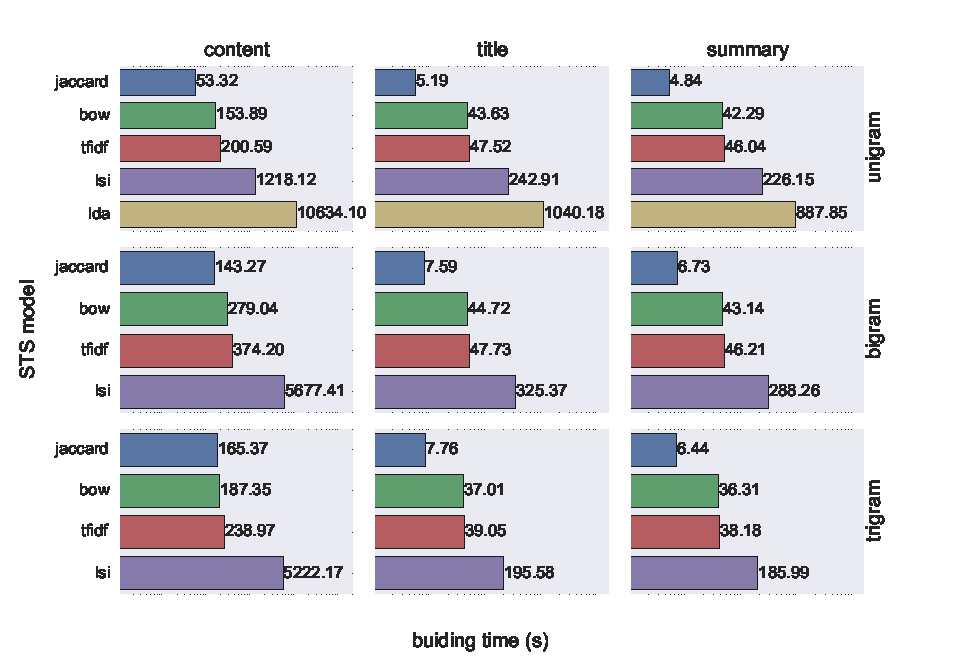
\includegraphics[width=\textwidth]{fig/building_time}
    \caption[Time cost (second) of building phase of Jaccard, BoW, \textit{tfidf}, LSI and LDA for all text fields over n-gram models]{Time cost (second) of building phase of Jaccard, BoW, \textit{tfidf}, LSI and LDA for all text fields over n-gram models. $73908$ candidate articles are used as training data to build the STS models.}
    \label{fig:build_time}
\end{figure}
\subsubsection{Comparison of predicting time}

The results of predicting time are illustrated in figure \ref{fig:predict_time} and analyzed as follows. 


\begin{itemize}
\item[1] Similar to building phase, \textit{Jaccard} is also quite different from other VSM methods. The \textit{Jaccard} similarity between two documents is computed by dividing the size of union of the corresponding term sets by the size of intersection of them. This operation is more costly than computing \textit{cosine} similarity between vectors. Compared with \tfidf{}, \textit{Jaccard} costs 20-fold, 10-fold and 21 fold time for \icontent{} in uni-, bi- and trigram, respectively.

\item[2] Predicting phase consists of representing phase and similarity computing phase. The first phase depends on the complexity of the corresponding model. Specifically, a document is represented as a vector of occurrence frequency, \tfidf{} weight or topic weight for BoW, \tfidf{} or topic models (i.e. LSI and LDA), respectively, and complexity increases progressively. The second phase depends on the vector dimension and the amount of vectors. Normally, the vector dimension of topic models is much lower than BoW and \tfidf{}, and hence, topic models cost less time in the second phase. In \icontent{}, the cost of LSI is similar to BoW and \tfidf{}, whereas it is much higher than BoW and \tfidf{} in \ititle{} and \isummary{}, which generate much smaller vocabularies and accordingly the lower dimension of term-weighted vectors. 

\end{itemize} 

\begin{figure}[!htb]
    \centering
    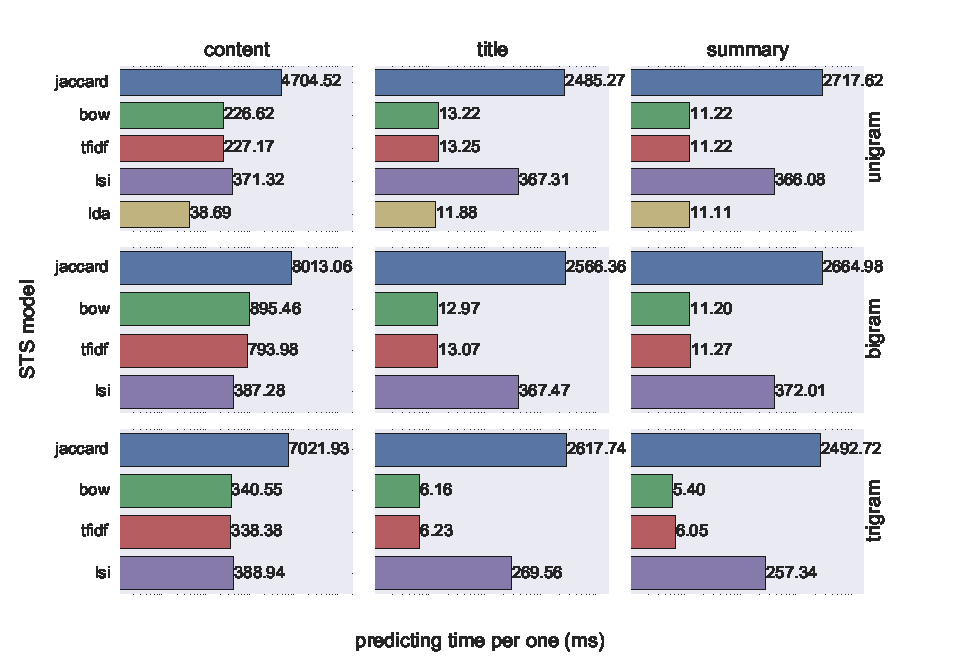
\includegraphics[width=\textwidth]{fig/predicting_time}
    \caption[Average time cost (millisecond) of selection of related articles per target]{Average time cost (millisecond) of selection of related articles per target. The operation consists of two phases: article transforming and similarity computing.}
    \label{fig:predict_time}
\end{figure}

In conclusion, we determine the final selection of the best STS methods for each PF in table \ref{tab:select}, taking into account both of effectiveness and efficiency. Besides the methods with the best effectiveness, LSI is selected for applying in \icontent{} over unigram, because LSI outperforms \tfidf{} in metric \textit{nDCG} and \textit{precision@2@h} with a larger $h$, and moreover, it is selected for analyzing the characteristics of topic models. \tfidf{} is also selected for applying in \icontent{} over trigram, because \tfidf{} is much more efficient than Jaccard, although its effectiveness is slightly lower than Jaccard. 

\begin{table}[!htb]
\centering
\small
\begin{tabularx}{0.8\textwidth}{|X|X|X|X|}
\hline
\textbf{Model} & \textbf{Content} & \textbf{Title} & \textbf{Summary} \\ \hline
\textbf{Unigram} & \tfidf{}/LSI & \tfidf{} & \tfidf{} \\ \hline
\textbf{Bigram} & \tfidf{} & \tfidf{} & \textit{Jaccard} \\ \hline
\textbf{Trigram} & \textit{Jaccard}/\tfidf{} & \textit{Jaccard} & \textit{Jaccard} \\ \hline
\end{tabularx}
\caption[Selection of STS methods for each text fields over n-gram models.]{Selection of STS methods for each text fields over n-gram models. For \icontent{} over unigram, LSI is also selected because of its better performance in metic \textit{nDCG} and \textit{precision@2@h} with a larger $h$. Meanwhile, \tfidf{} is also chosen in \icontent{} over trigram because of its efficient with $21 \times$ speed compared with Jaccard in predicting phase} 
\label{tab:select}
\end{table}


\subsection{Results of Incremental Updating}
\label{sec:5.4}

As described in section \ref{sec:4.4}, the whole corpus is splitted into a historic dataset, in which the articles are released before 2012 and which is used for initializing the system, and a testing dataset containing the released after 2012 articles, which is used for both of evaluating the system and updating the system incrementally. In the sight of reality, the candidates of related articles for a target article must be released before the target. We have two main purposes of the experiment. On the one hand, we attempt to find the differences between the results of the system with incremental updating and the results of the controlled experiments and analyse whether the differences are acceptable and the reason why the differences occur. On the other hand, we focus on the trade-off between the step of updating and the corresponding additional cost of time. 

Before analyzing the results, we define the controlled experiments in advance. The system in the controlled experiments is constant. It means, the systems are trained only in the phase of initialization and keep constant after that. In the first experiment, the STS methods in the system is learned from the candidate corpus, or, in other words, the released before 2012 articles. Accordingly the system contains only the semantic information before the first target is released and this system is hence ``out-of-date''. The system 1 is called the ``lower bound'' system. In the second experiment, there is only one difference from the first experiment, that the STS methods are trained by the all complete articles and the system contains therefore the complete semantic information of the entire corpus. The second controlled system is a ``upper bound'' system. Any article which is released before the target is transformed as the corresponding representation by the STS methods.  The comparison between the evaluated system and the controlled systems is able to indicate the particular characteristics of the system with incremental updating and the differences from the ``out-of-date'' system and ``coverall'' system. 

Jaccard and BoW are not involved in the evaluation. These two methods are only dependent on the current articles and independent of the rest information of the corpus. The model updating therefore does not affect the results of the semantic similarity from Jaccard and BoW. Consequently, the evaluation concentrates on three VSMs, namely tf-idf and LSI (due to the high complexity and low performance, LDA is ignored). Based on the result of experiment 1, the preprocessed field \icontent{} with unigram always outperforms other preprocessed fields. In this experiment, we only discuss the performance of the three STS methods in \icontent{} with unigram. 

\subsubsection{Effectiveness}

Instead of \textit{precision@k@h} used in experiment 1, we compute the precision with moving average, which is often applied with time series data to smooth out short-term fluctuations and highlight longer-term trends or cycles. A typical application of moving average is to analyze stock prices. In our case, we calculate the moving mean precision (MMP) of the $i$-th target article and $n-1$ previous targets mathematically as follows:

\begin{figure}[!htb]
    \centering
    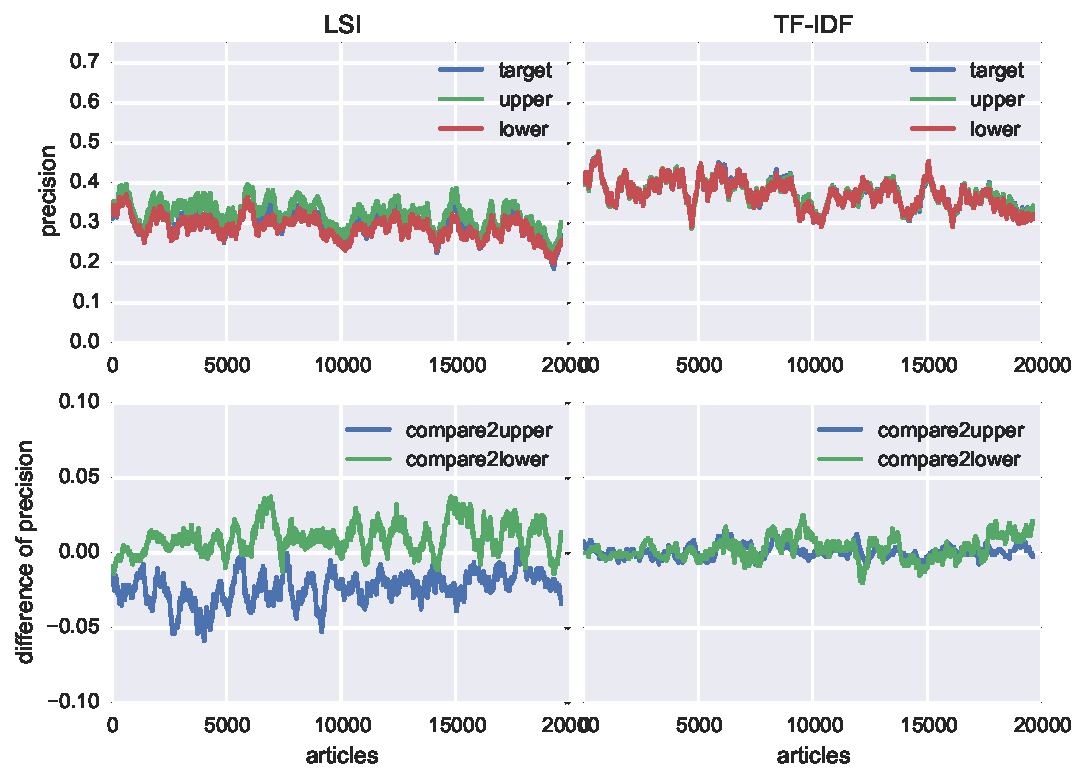
\includegraphics[width=\textwidth]{fig/precision_inc}
    \caption[Moving average precision of the evaluated system with the controlled systems]{Moving average precision of the evaluated system with the controlled systems. The window size of moving average is set to $400$. The upper sub-figures illustrate the precision plots of the evaluated, upper and lower systems with the color of blue, green and red, respectively. The bottom sub-figures show the plots of subtracting the precision of the upper and lower systems from the precision of the evaluated system, respectively.}
    \label{fig:predict_inc}
\end{figure}

\clearpage

\begin{equation}
    MM_{i} = \frac{\sum^{n-1}_{j=0} \text{correct predictions for }(i-j)}{k\times n}
\end{equation}


where $n$ is the moving window size and pre-defined as $100$ and $k$ is the number of related articles for each target. 

Figure \ref{fig:predict_inc} illustrates the moving average precision of the evaluated system and the controlled systems. In general, the average precision of the system using LSI and \tfidf{} is $29.95\%$ and $37.50\%$, respectively. The result confirms the conclusion which we obtain in experiment 1. The subfigures below is obtained by subtracting the precision of the controlled systems from the precision of the evaluated system. For method LSI, the evaluated system outperforms the ``lower bound'' system and underperforms the ``upper bound'' system definitely. Meanwhile, the differences in the systems using \tfidf{} are insignificant. Therefore, LSI is more sensitive than \tfidf{} to the completeness of information and model updating. Furthermore, for LSI, the difference between the evaluated system and the ``lower bound'' system keeps increasing along with handling more and more articles, and the difference between the evaluated system and the ``upper bound'' system is in the decreasing trend. 

The effectiveness of the system is dependent on the scale of the corpus, from which the system is trained. In the real world application, the judgements of related articles for all articles can be updated every quarter or every half year, such that the system can discover related articles more precisely. 


\subsubsection{Efficiency}

\begin{figure}[!htb]
    \centering
    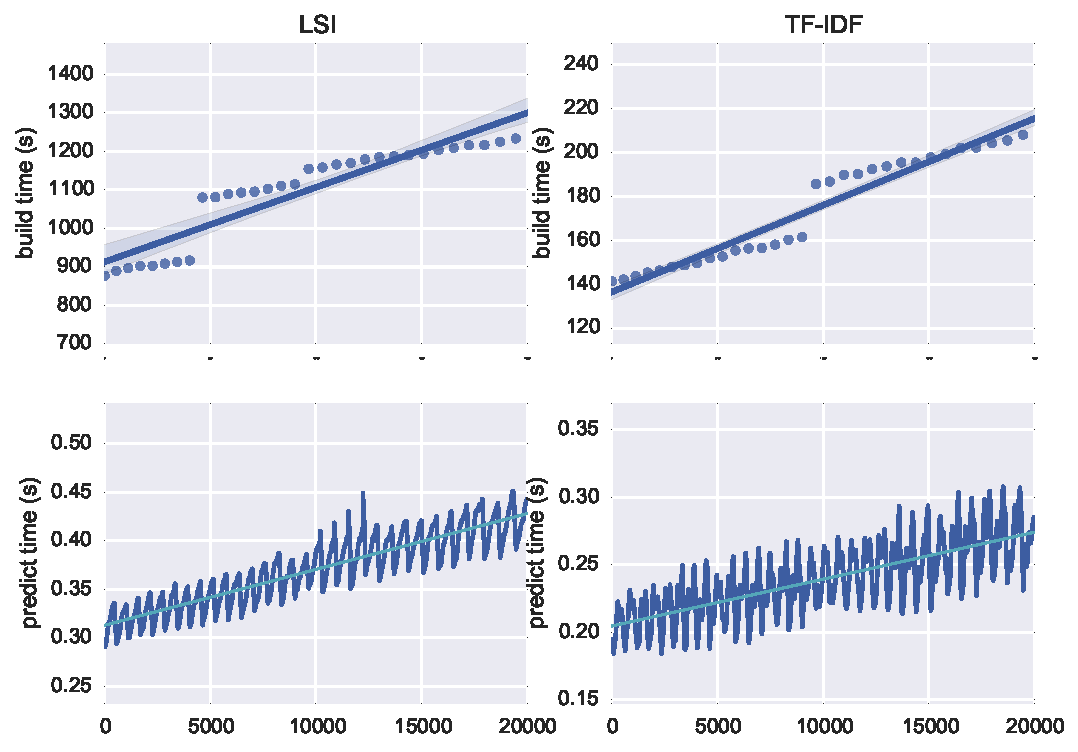
\includegraphics[width=\textwidth]{fig/runtime_inc}
    \caption[Efficiency of the evaluated system with incremental updating]{Efficiency of the evaluated system with incremental updating. The upper sub-figures show the time cost of building phase for each time of updating. The scatter plots are drawn with the practically consumed time (second) and the line plots are drawn by the linear regression to depict future time cost. The bottom sub-figures show the time cost of predicting phase. The plots with the color of blue are created by the practically consumed time and the plots with the color of bluish green are generated by the linear regression to depict the growth trends. }
    \label{fig:runtime_inc}
\end{figure}

Figure \ref{fig:runtime_inc} reports the time cost of building and predicting for the system using LSI and \tfidf{} respectively. The analysis of the reports is given as follows:

\begin{itemize}
    \item The time cost of model building and related articles predicting keeps linear increasing, since the candidate dataset keeps growing. For method LSI, the building time and predicting time increase by $19.3$ seconds and $5.8$ milliseconds, respectively, with the size of candidates increased by $1000$. Meanwhile, for method \tfidf{}, the building time and the predicting time increase by $4.0$ seconds and $3.5$ milliseconds with the size of candidates increased by $1000$, respectively. LSI is slower than \tfidf{} in both of building and predicting. 
    \item The jitter of predicting time is caused by the implementation. As an article is stored in the system, the system puts it at first into a temporary collection. The temporary collection will be merged into the candidate dataset. The similarity computation with articles in the candidate dataset is much more efficient than the computation of similarity with articles in the temporary collection. That is why the predicting time increases significantly before next updating and decreases to the normal level after updating. 
    
\end{itemize}

\bigbreak

\subsection{Error Analysis}
\label{sec:5.5}

We present insights on the most severe types of errors of false positive and false negative that occurred in the experiments. In order to confirm the reasons or conditions of the errors, we inspect manually the predictions of the framework to discover related articles and compare them with the golden standard understanding of human beings.  

\subsubsection{False Positive Error}

A false positive error is a result that indicates a given condition has been fulfilled, when it actually has not been fulfilled. In our case, a false positive error is the event that an article which is actually unrelated to the target article is assigned as related by the framework. 

\begin{itemize}
    \item One type of fp errors is caused by the labeled corpus we select. The list of related articles is marked by the editor manually and the size is limited up to $2$. Therefore, the list is incomplete, so that articles which should be related to each other under human understanding are unreachable to each other in the related-graph generated based on the lists of related articles. Only this type is not the real errors but the inherent systematic lack. 
    
    Example: 
    \begin{itemize}
        \item \textit{``Tod dem Diktator'' - Rufe zur Vereidigung} (\textit{``Death to the dictator'' - require for swearing}) \footnote{\url{http://www.zeit.de/online/2009/32/iran-proteste-vereidigung}}
        \item \textit{Proteste in Teheran dauern an} (\textit{Protests in Tehran persist}) \footnote{\url{http://www.zeit.de/online/2009/32/iran-ahmadineschad-proteste}}
    \end{itemize}
    The both articles report the protest against Mahmoud Ahmadinejad, who is re-elected as the Iranian president, and the international as well as authoritative reaction. The articles should be related by the human judgement, but there is no related-path between them. We consider that the incompleteness of labeling causes the fp error. 
    
    \item One article usually contains a set of topics rather than the single topic. The topics are not treated equally, but they are understood in different importance. It is complicate and subtle, how human beings weigh the importance of different topics. Out of this view point, two articles are assigned as related, only when they share the topics with the highest weight, otherwise they are unrelated, even though they are similar to each other in semantic or lexical meaning. 
    
    Example:
    \begin{itemize}
        \item \textit{Tunesiens Innenminister wird neuer Regierungschef} (\textit{Tunisia Interior Minister appointed new head of government}) \footnote{\url{http://www.zeit.de/politik/ausland/2013-02/tunesien-regierungschef-larayedh-jebali}}
        \item \textit{Tunesien hebt den Ausnahmezustand seit Arabellion auf} (\textit{Tunisia cancels the state of emergency beginning from Arabellion}) \footnote{\url{http://www.zeit.de/politik/ausland/2014-03/tunesien-ausnahmezustand-aufhebung}}
    \end{itemize}
    
    The both articles mention the identical background, subject of the events and keywords. However, the critical reported topics are different and unrelated. In addition, quite a few named entities which they share confuse the framework predicts the relatedness between them. 
    
    \item Two articles have the identical or similar information, but they mention the very different topics. 
    Example: 
    \begin{itemize}
        \item \textit{Dem Pr\"asidentenpaar droht eine herbe Wahlniederlage} (\textit{The presidential couple threatens a bitter election defeat}) \footnote{\url{http://www.zeit.de/online/2009/27/argentinien-wahl-kirchner}}
        \item \textit{Der Schattenpr\"asident} (\textit{The Shadow President}) \footnote{\url{http://www.zeit.de/politik/ausland/2010-10/nestor-kirchner-nachruf}}
    \end{itemize}
    The articles report the politics in Argentina and use many similar or same words to describe the situation of the government and the action thereof. However, the first article focuses on the difficulty of election, while the second article reviews mainly the record of achievements of the former president who just died. Hence, they are unrelated very clearly. 
    
    \item Two articles are about entirely different field and totally unrelated. 
    
    Example: 
    \begin{itemize}
        \item \textit{Ohne Gras kein Spa\ss{}} (\textit{Without grass no fun}) \footnote{\url{http://www.zeit.de/2009/20/Portugal-Golf}}
        \item \textit{Jonglieren entspannt und macht schlau} (\textit{Juggling relaxed and makes you smart}) \footnote{\url{http://www.zeit.de/karriere/beruf/2012-10/konzentration-gehirnleistung-jonglage}}
    \end{itemize}
    
    The first article describes the experiences of the golf trip in Portugal, whereas the second article reports a kind of game in office which can make the participants relaxer and smarter. They belong to even different separated categories and cannot be related to each other. 
\end{itemize}

\subsubsection{False Negative Error}

A false positive error is, in our case, a result that indicates an article which is actually quite related to the target article is judged with a very low relatedness degree. Now we consider that the articles which are very related to the target article are exactly predicted unrelated with an unexpected low relatedness degree. More specifically, we only inspect the extreme and typical error that the framework treats the articles which are directly adjacent to the target article in the related-graph and should be one of the most related articles as unrelated in a very low level. We discuss the characteristics of the errors and the reasons why the errors occur. 

\begin{itemize}
    \item Two articles discuss the same topics and related meaning, but the points of view and concrete events are different. 
    
    Example:
    \begin{itemize}
    \item \textit{Drittmittel sind ungleich verteilt} (\textit{Third-party funds are distributed unequally}) \footnote{\url{http://www.zeit.de/studium/hochschule/2014-02/Drittmittel-an-Hochschulen}}
    \item \textit{Uni Leipzig droht mit Schlie\ss{}ung ganzer Fakult\"aten} (\textit{Uni Leipzig threatened with closure of entire faculties}) \footnote{\url{http://www.zeit.de/studium/hochschule/2014-02/universitaet-leipzig-finanzierung}}
    \end{itemize}
    The first article discusses the phenomenon of education abstractly, while the second reports the very concrete expression in a specific university. They are not similar semantically, but related because of the same topic.
    
    
    \item Humans classify an articles into topics hierarchically rather than separately. Two articles may be related in higher level but different in the particular level. The critical point is how the humans determine which level is the most important. 
    
    Example:
    \begin{itemize}
        \item \textit{Der Jugendschutzfilter blockiert zu viel} (\textit{The youth safety filter blocking too much}) \footnote{\url{http://www.zeit.de/digital/internet/2012-02/jugendschutzfilter-filtern-blogs}}
        \item \textit{Filmwirtschaft weitet Selbstkontrolle auf Internet aus} (\textit{Film industry is expanding self-regulation on the Internet}) \footnote{\url{http://www.zeit.de/kultur/film/2011-10/fsk-jugendschutz-internet}}
    \end{itemize}    
    
    The first article reports the current situation of the youth safety filter and the second article reports that the change of film industry on the Internet may harm the youth protection. These two article share the same topic on ``youth procection'' but have difference on the particular fields. They are labeled as related based on the editor's understanding. However, this judgement is not absolutely correct. 
    
\end{itemize}


%\subsection{Conclusion}
%\label{sec:5.6}
%1. 分析了性能,分析了错误
%2. 最好的是content-1-tfidf,其他的见表格
%3. 问题是没有使用corpus中的标记,即保存的人工标记related。利用这些数据,会训练出更加specific更加precise的模型,在下一章详细说明。